\documentclass[tikz,border=0pt,11pt]{standalone}
\usepackage[T1]{fontenc}
\usepackage[utf8]{inputenc}
\usepackage{lmodern,amsmath,amssymb}
\usepackage[swedish]{babel}
\usetikzlibrary{arrows.meta,calc,positioning,decorations.pathmorphing,decorations.pathreplacing,patterns,shadings}
\definecolor{navy}{HTML}{102F40}
\definecolor{teal}{HTML}{147D78}
\definecolor{lightteal}{HTML}{E6F1ED}
\definecolor{gold}{HTML}{B88B3B}
\definecolor{palegold}{HTML}{F7EEDB}
\definecolor{rust}{HTML}{B6533B}
\definecolor{palerust}{HTML}{FAEAE4}
\definecolor{paper}{HTML}{F7F5EE}
\definecolor{muted}{HTML}{5B6D72}
\definecolor{line}{HTML}{D6DED8}
\renewcommand{\familydefault}{\sfdefault}
\newcommand{\atom}[5]{\shade[ball color=#3!70] (#1,#2) circle (#5);\node[text=white,font=\bfseries\small] at (#1,#2){#4};}
\newcommand{\water}[3]{\begin{scope}[shift={(#1,#2)},scale=#3]\draw[navy!45,line width=2pt] (-.3,.22)--(0,0)--(.3,.22);\atom{0}{0}{rust}{O}{.22}\atom{-.3}{.22}{teal}{H}{.15}\atom{.3}{.22}{teal}{H}{.15}\end{scope}}
\newcommand{\panel}[4]{\filldraw[fill=white,draw=line,rounded corners=5pt] (#1,#2) rectangle ++(#3,#4);}
\newcommand{\note}[4]{\node[txt,text width=#3cm] at (#1,#2){#4};}
\tikzset{txt/.style={anchor=north west,align=left,text=navy,font=\small},
 head/.style={anchor=west,text=navy,font=\bfseries\large},
 label/.style={align=center,text=navy,font=\small},
 smalllabel/.style={align=center,text=muted,font=\footnotesize},
 arrow/.style={-{Latex[length=2.5mm,width=1.8mm]},line width=1.2pt,draw=teal},
 goldarrow/.style={-{Latex[length=2.5mm]},line width=1.2pt,draw=gold},
 rustarrow/.style={-{Latex[length=2.5mm]},line width=1.2pt,draw=rust},
 dashedarrow/.style={arrow,dashed},
 badge/.style={fill=lightteal,rounded corners=3pt,text=teal,font=\bfseries\small,inner sep=5pt}}
\begin{document}
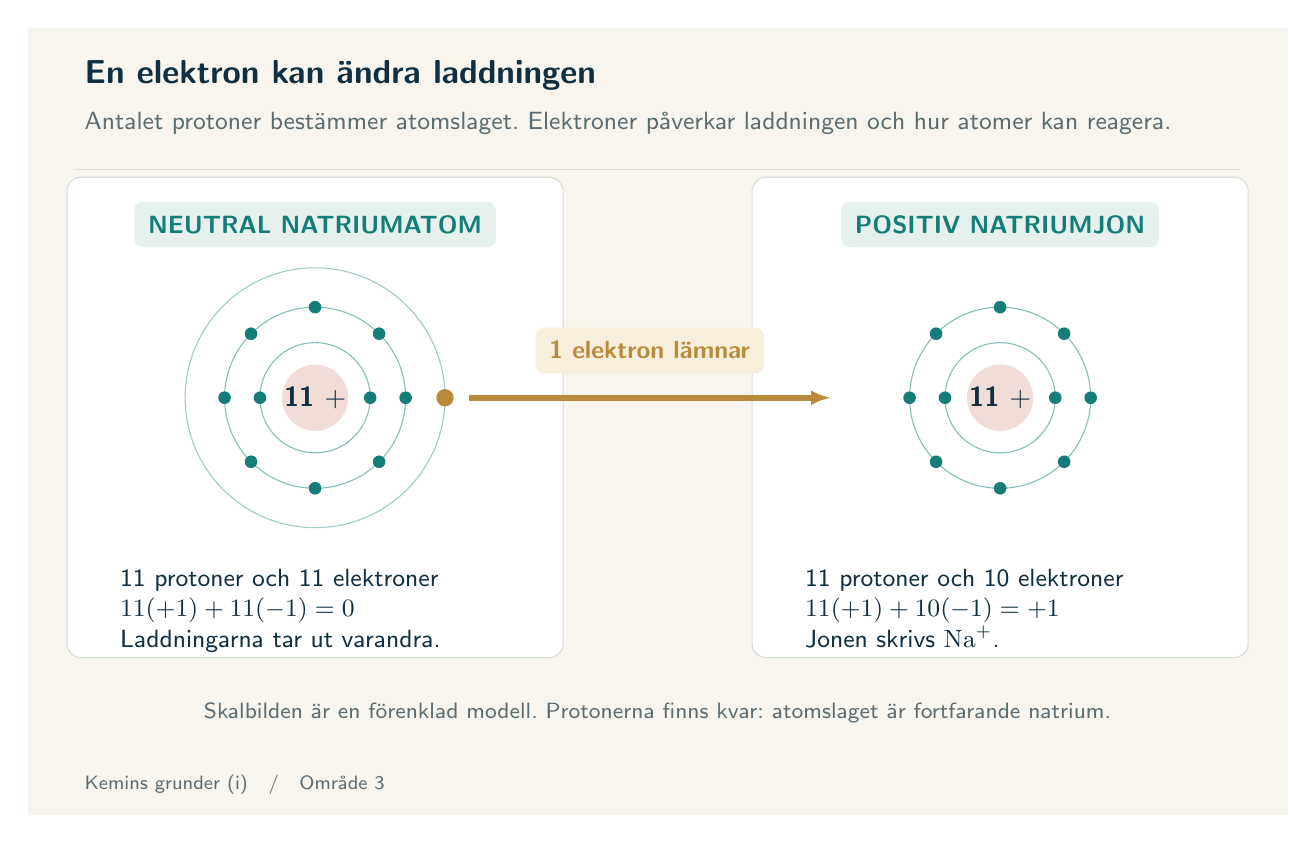
\begin{tikzpicture}[x=1cm,y=1cm]
\path[use as bounding box] (0,0) rectangle (16,10);
\fill[paper] (0,0) rectangle (16,10);
\node[head] at (.6,9.4){En elektron kan ändra laddningen};
\note{.6}{9.05}{14.8}{\textcolor{muted}{Antalet protoner bestämmer atomslaget. Elektroner påverkar laddningen och hur atomer kan reagera.}}
\draw[line] (.6,8.2)--(15.4,8.2);

\panel{.5}{2}{6.3}{6.1}\panel{9.2}{2}{6.3}{6.1}
\node[badge] at (3.65,7.5){NEUTRAL NATRIUMATOM};\node[badge] at (12.35,7.5){POSITIV NATRIUMJON};
\foreach \cx in {3.65,12.35}{\foreach \r in {.7,1.15}{\draw[teal!50] (\cx,5.3) circle(\r);} \fill[rust!20] (\cx,5.3) circle(.42);\node[label,font=\bfseries] at (\cx,5.3){11 $+$};}
\foreach \a in {0,180}{\fill[teal] ($(3.65,5.3)+(\a:.7)$) circle(.08);\fill[teal] ($(12.35,5.3)+(\a:.7)$) circle(.08);}
\foreach \a in {0,45,...,315}{\fill[teal] ($(3.65,5.3)+(\a:1.15)$) circle(.08);\fill[teal] ($(12.35,5.3)+(\a:1.15)$) circle(.08);}
\draw[teal!40] (3.65,5.3) circle(1.65);\fill[gold] (5.3,5.3) circle(.11);
\draw[goldarrow,line width=2pt] (5.6,5.3)--(10.2,5.3);\node[badge,fill=palegold,text=gold] at (7.9,5.9){1 elektron lämnar};
\note{1.05}{3.25}{5.25}{11 protoner och 11 elektroner\par $11(+1)+11(-1)=0$\par Laddningarna tar ut varandra.}
\note{9.75}{3.25}{5.25}{11 protoner och 10 elektroner\par $11(+1)+10(-1)=+1$\par Jonen skrivs $\mathrm{Na^+}$.}
\node[smalllabel,text width=14cm] at (8,1.3){Skalbilden är en förenklad modell. Protonerna finns kvar: atomslaget är fortfarande natrium.};\node[anchor=west,text=muted,font=\scriptsize] at (.6,.38){Kemins grunder (i)\quad /\quad Område 3};

\end{tikzpicture}\end{document}
